\documentclass[11pt]{iopart}
\usepackage[english]{babel}
\pdfoutput=1
%\usepackage{amsmath}
\usepackage{wasysym}
\usepackage{booktabs}
\usepackage{amssymb}
\usepackage{amsbsy}
\usepackage{verbatim}
\usepackage{graphicx}
\usepackage{epstopdf}
\usepackage{color}
\usepackage{sidecap}
\usepackage{bm}% bold math

\usepackage[colorlinks,bookmarks=false,citecolor=blue,linkcolor=red,urlcolor=blue]{hyperref}

%\usepackage{cite}

%
% WARNING !!!!
% 
% iopart.cls definition of \tableofcontents overwrites the
% short title printed every page. 
% The following redefinition of \tableofcontents fixes the
% the problem. 

\catcode`@=11 % If we need private TeX macros
\renewcommand\tableofcontents{%
  \section*{\contentsname}%
  \@starttoc{toc}%
}
\catcode`@=12% '@' is no more a character
\newcommand{\bra}[1]{\langle\left.{#1}\right|}
\newcommand{\ket}[1]{\left|{#1}\right.\rangle}


\def\be{\begin{equation}}
\def\ee{\end{equation}}
\def\u{\uparrow}
\def\d{\downarrow}
\def\nm{\newmoon}
\def\fm{\fullmoon}
\def\T{\rule{0pt}{.6cm}}
\def\B{\rule[-.4cm]{0pt}{0pt}}

\begin{document}

\setlength{\parindent}{0pt}


\title{Finite-size study of the Quench Action approach in integrable spin 
chains}

\author{Vincenzo Alba$^1$, Pasquale Calabrese$^1$}
\address{$^1$ International School for Advanced Studies (SISSA),
Via Bonomea 265, 34136, Trieste, Italy,
INFN, Sezione di Trieste}


\date{\today}



%%%%%%%%%%%%%%%%%%%%%%%%%%%%%%%%%%%%%%%%%%%%%%%%%%%%%%%%%%%%%%%%%%%%%%%%%%
\begin{abstract} 


fdasfa
\end{abstract}

\maketitle

%%%%%%%%%%%%%%%%% INTRODUCTION %%%%%%%%%%%%%%%%%%%%%
\section{Introduction}
\label{intro}

We show that it is possible to numerically simulate the Quench Action approach 
combining Monte Carlo methods and Bethe ansatz techniques. 

We focus on the situation in which the pre-quench initial state is the Neel 
state or the Majumdar-Ghosh state. 

We investigate the importance of the zero-momentum strings in the Quench Action. 

Without zero-momentum strings the overlap saturation rules are not valid, 
i.e., in finite size systems the vast majority of the eigenstates contain 
zero momentum strings. 

The details on the eigenstates counting depend on the pre-quench initial state. 

However, we show that one can restrict to the set of non-zero momentum strings. 
The fact that one neglects zero-momentum strings gives rise only to scaling 
corrections. 

We also investigate the validity of the Bethe-Takahashi approximation for the 
calculation of the overlap. 

%%%%%%%%%%%%%%%%%%%%%%% BETHE ANSATZ APPROACH %%%%%%%%%%%%%%%%%%%%%%%%%%%%%%
\section{The Heisenberg spin chain}
\label{xxx-chain}

Here we consdier the spin-$\frac{1}{2}$ isotropic Heisenberg chain ($XXX$ chain). 
The $XXX$ chain with $L$ sites is defined by the Hamiltonian 
%
\begin{equation}
\label{xxx-ham}
{\mathcal H}\equiv J\sum\limits_{i=1}^L\left[\frac{1}{2}(S_i^+S^-_{i+1} 
+S_i^{-}S_{i+1}^+)+S_i^zS_{i+1}^z\right],  
\end{equation}
%
where $S^{\pm}_i\equiv (\sigma_i^x\pm i\sigma_i^y)/2$ are spin operators acting on the 
site $i$, $S_i^z\equiv\sigma_i^z/2$, and $\sigma^{x,y,z}_i$ the Pauli matrices. We fix 
$J=1$ and use periodic boundary conditions, identifying sites $L+1$ and $1$. The total 
magnetization $S_{T}^z\equiv\sum_iS_i^z=L/2-M$, with $M$ number of down spins (particles), 
commutes with~\eref{xxx-ham}, and it is here used to label its eigenstates. 

%%%%%%%%%%%%%%%%%%%%%%%%%%%%%%%%%%%%%%%%%%%%%%%%%%%%%%%%%%%%%%%%%%%%%%%%%%%
\subsection{Bethe equations and wavefunctions}
\label{bethe_equations}

The generic eigenstate of~\eref{xxx-ham} in the sector with $M$ particles can be written as 
%
\begin{equation}
\label{ba_eig}
|\Psi_M\rangle=\sum\limits_{1\le x_1<x_2<\dots<x_M\le L}A_M(x_1,x_2,
\dots,x_M)|x_1,x_2,\dots,x_M\rangle,
\end{equation}
%
where the sum is over the positions $\{x_i\}$ of the particles, and $A_M(x_1,
x_2,\dots,x_M)$ is the eigenstate amplitude corresponding to particles 
at positions $x_1,x_2,\dots, x_M$. $A_M(x_1,x_2,\dots, x_M)$ is given as 
%
\begin{equation}
\label{ba_amp}
A_M(x_1,x_2,\dots,x_M)\equiv\sum\limits_{{\mathcal P}\in S_M}\exp\Big[i
\sum\limits_{j=1}^Mk_{{\mathcal P}_j}x_j+i\sum\limits_{i<j}\theta_{{
\mathcal P}_i{\mathcal P}_j}\Big].
\end{equation}
%
Here the outermost sum is over the permutations $S_M$ 
of the so-called quasi-momenta $\{k_1,k_2,\dots,k_M\}$. The two-particle 
scattering phases $\theta_{m,n}$ are defined as 
%
\begin{equation}
\label{s_phases}
\theta_{m,n}\equiv \frac{1}{2i}\log\Big[-\frac{e^{ik_m+ik_n}-2e^{ik_m}+1}
{e^{ik_m+ik_n}-2e^{ik_n}+1}\Big].
\end{equation}
%
The energy associated to the eigenstate~\eref{ba_eig} is  
%
\begin{equation}
\label{ba_ener}
E=\sum\limits_{\alpha=1}^M(\cos(k_\alpha)-1).
\end{equation}
%
The quasi-momenta $\{k_\alpha\}$ are obtained by solving the so-called 
Bethe equations  
%
\begin{equation}
\label{ba_eq}
e^{ik_\alpha L}=\prod\limits^M_{\beta\ne\alpha}\Big[-\frac{1-2e^{
ik_\alpha}-e^{ik_\alpha+ik_\beta}}{1-2e^{ik_\beta}-e^{ik_\alpha+
ik_\beta}}\Big].
\end{equation}
%
It is useful to  introduce the rapidities $\{\lambda_\alpha\}$ as 
%
\begin{equation}
\label{rap}
k_\alpha=\pi-2\arctan(\lambda_\alpha)\quad\mbox{mod}\, 2\pi.
\end{equation}
%
Taking the logarithm on both sides in~\eref{ba_eq}, and using~\eref{rap}, 
one obtains the Bethe equations in logarithmic form as 
%
\begin{equation}
\label{ba_eq_log}
\arctan(\lambda_\alpha)=\frac{\pi}{L}J_\alpha+\frac{1}{L}\sum\limits_{
\beta\ne\alpha}\arctan\Big(\frac{\lambda_\alpha-\lambda_\beta}{2}\Big),
\end{equation}
%
where $-L/2<J_\alpha\le L/2$ are the so-called Bethe quantum numbers. The 
$J_\alpha$ are half-integers and integers for $L-M$ even and odd. 


These solutions of the Bethe equations~\eref{ba_eq} form particular ``string'' patterns 
in the complex plane, in the limit of large chains $L\to\infty$(string hypothesis)~\cite{
bethe-1931,taka-book}. Specifically, rapidities forming a ``string'' of length $1\le 
n\le M$ (that we defined here as $n$-string) are parametrized as 
%
\begin{equation}
\label{str_hyp}
\lambda^{j}_{n;\gamma}=\lambda_{n;\gamma}-i(n-1-2j)+i\delta_{n;\gamma}^j,\qquad 
j=0,1,\dots, n-1, 
\end{equation}
%
where $\lambda_{n;\gamma}$ is the real part of the string (string center), 
and $\gamma$ labels strings with different centers, while $j$ labels the different 
components of the string. In~\eref{str_hyp} $\delta_{n;\gamma}^j$ are the string 
deviations, which typically vanish exponentially in the thermodynamic limit. 

Notice that pure real rapidities are strings of unit length ($1$-strings). 


\subsection{Bethe-Takahashi equations.} 

The string centers $\lambda_{n;\gamma}$ in~\eref{str_hyp} are obtained by solving the 
so-called Bethe-Takahashi equations
%
\begin{equation}
\label{bt_eq}
2L\theta_n(\lambda_{n;\gamma})=2\pi I_{n;\gamma}+\sum\limits_{(m,
\beta)\ne(n,\gamma)}\Theta_{m,n}(\lambda_{n;\gamma}-\lambda_{m;\beta}), 
\end{equation}
%
where the generalized scattering phases $\Theta_{m,n}$ read 
%
\begin{eqnarray}
\nonumber\fl\Theta_{m,n}(x)\equiv\left\{\begin{array}{cc}
\theta_{|n-m|}(x)+\!\!\!\!\!\sum
\limits_{r=1}^{(n+m-|n-m|-1)/2}\!\!\!\!\!2\theta_{|n-m|+2r}(x)
+\theta_{n+m}(x) & \quad\mbox{if}
\quad n\ne m\\\fl\sum\limits_{r=1}^{n-1}2\theta_{2r}(x)+
\theta_{2n}(x) & \quad\mbox{if}\quad n=m
\end{array}\right.
\end{eqnarray}
%
and $\theta_\alpha(x)\equiv 2\arctan(x/\alpha)$. Here $I_{n;\gamma}$ are the 
Bethe-Takahashi quantum numbers associated with $\lambda_{n;\gamma}$. 

Each $M$-particle eigenstate can be characterized by its ``string content'' ${
\mathcal S}\equiv\{s_1,\dots,s_M\}$, with $s_n$ the number of $n$-strings. 

It can be shown that $I_{n;\gamma}$  are integers or half-integers for $L-s_n$ 
odd and even, respectively. 


Clearly, the constraint $\sum_{\alpha=1}^{M}\alpha s_\alpha=M$ 
has to be satisfied. The upper bound for the Bethe-Takahashi quantum numbers 
can be derived as   
%
\begin{equation}
|I_{n;\gamma}|\le I^{(MAX)}_{n}\equiv\frac{1}{2}(L-1-\sum
\limits_{m=1}^Mt_{m,n}s_m),
\label{bt_qn_bound}
\end{equation}
%
where $t_{m,n}\equiv 2\mbox{min}(n,m)-\delta_{m,n}$. 



%%%%%% NEEL OVERLAP
\section{Overlap with the Neel state}


Here we restrict to the parity-invariant eigenstates. These are the only 
eigenstates with non-zero overlap with the Neel state. Parity-invariant 
eigenstates contain only pairs of rapidities with opposite sign.  

We denote the generic parity invariant eigenstate as $|\{\pm\lambda_j\}_{j=1}^m,
n_\infty\rangle$, where $m$ is the number of rapidity pairs, $N_{\infty}$ is the 
number of infinite rapidities, with $M=L/2=N_\infty+2m$, and $n_\infty\equiv 
N_\infty/L$ is the density of infinite rapidities. 

The overlap with the Neel state $|N\rangle$ reads 
%
\begin{equation}
\label{neel-ov}
\frac{\langle N|\{\pm\lambda_j\}_{j=1}^m,n_\infty\rangle}{|||\{\lambda_j\}_{j=1}^m,
n_\infty\rangle||}=\frac{\sqrt{2}N_{\infty}!}{\sqrt{(2N_\infty)!}}\left[\prod_{j=1}^m
\frac{\sqrt{\lambda_j^2+1}}{4\lambda_j}\right]\sqrt{\frac{\textrm{det}_m(G^+)}{
\textrm{det}_m(G^-)}}
\end{equation}
%
where 
%
\begin{equation}
\label{G-pm}
G^{\pm}_{jk}=\delta_{jk}\Big(NK_{1/2}(\lambda_j)-\sum\limits_{l=1}^mK_1^+(\lambda_j,
\lambda_l)\Big)+K_{1}^{\pm}(\lambda_j,\lambda_k),\quad\,j,k=1,\dots,m
\end{equation}
%
and 
%
\begin{equation}
\label{K-1}
K_1^\pm(\lambda,\mu)=K_1(\lambda-\mu)\pm K_1(\lambda+\mu)
\end{equation}
%
and 
%
\begin{equation}
\label{K-alpha}
K_\alpha(\lambda)\equiv\frac{8\alpha}{\lambda^2+4\alpha^2}
\end{equation}
%

%%%%%% REDUCED NEEL OVERLAP
\subsection{Reduced Neel overlap}

Here we consider the overlap formula for the Neel state~\eref{neel-ov} in the 
limit $L\to\infty$, assuming that the rapidities form perfect strings.  

In the case of perfect strings the matrices $G^{\pm}_{jk}$ become ill-defined. 
Precisely, $K_{1}^\pm(\lambda,\mu)$ diverges if $\lambda$ and $\mu$ are successive 
members of the same string, i.e., $|\lambda-\mu|=2i$.  

It is possible to rewrite~\eref{neel-ov} in terms of the string centers 
$\lambda_{n;\alpha}$ only. Here we restrict ourselves to rapidity configurations 
with no zero-momentum strings. Our results are not valid for zero-rapidity 
strings. These would require the knowledge of the precise form of the string 
deviations, i.e., the dependence of the string deviations on $L$, as it has 
been pointed out in Ref.~\cite{calabrese-2014}. 

It is convenient to split the indices $i,j$ of $G^\pm_{ij}$ as $i=(n,\alpha)$ 
$j=(m,\beta)$, with $n,m$ being the length of the strings and $\alpha,\beta$ 
labelling the string centers. 

The result reads 
%
\begin{equation}
\fl \frac{1}{2}G^+_{(n,\alpha)(m,\beta)}=\left\{\begin{array}{cc}
L\theta_n'(\lambda_{n;\alpha})
-\sum\limits_{(\ell,\gamma)\ne(n,\alpha)}(\Theta'_{n,\ell}
(\lambda_{n;\alpha}-\lambda_{\ell;\gamma})+\Theta'_{n,\ell}
(\lambda_{n;\alpha}+\lambda_{\ell;\gamma})) & \textrm{if}\,(n,\alpha)= (m,\beta)\\
\Theta'_{n,m}
(\lambda_{n;\alpha}-\lambda_{m;\beta})+\Theta'_{n,m}
(\lambda_{n;\alpha}+\lambda_{m;\beta}) & \textrm{if}\,(n,\alpha)\ne(m,\beta)
\end{array}\right.
\end{equation}
%
Here $\theta_n'(x)\equiv d/dx \theta_n(x)=2n/(n^2+x^2)$ and $\Theta'(x)\equiv d/dx
\Theta(x)$. 

For $G^-_{ij}$ one obtains 

\begin{equation}
\fl\frac{1}{2}G^-_{(n,\alpha)(m,\beta)}=\left\{\begin{array}{cc}
(L-1)\theta'_n(\lambda_{n;\alpha})-2\sum\limits_{k=1}^{n-1}\theta'_k(\lambda_{n;\alpha})
-\sum\limits_{(\ell,\gamma)\ne(n,\alpha)}(\Theta'_{n,\ell}
(\lambda_{n;\alpha}-\lambda_{\ell;\gamma})+\Theta'_{n,l}
(\lambda_{n;\alpha}+\lambda_{\ell;\gamma})) & \quad\textrm{if}\,(n,\alpha)= (m,\beta)\\
\Theta'_{n,m}
(\lambda_{n;\alpha}-\lambda_{m;\beta})-\Theta'_{n,m}
(\lambda_{n;\alpha}+\lambda_{m;\beta})) & \quad\textrm{if}\,(n,\alpha)\ne(m,\beta)
\end{array}\right.
\end{equation}
%
Finally, the multiplicative prefactor in~\eref{neel-ov} for the generic $n$-string 
can be rewritten as 
%
\begin{equation}
\prod\limits_{a=1}^n\frac{\sqrt{(\lambda^a_{n;\alpha})^2+1}}{4\lambda^a_{n;\alpha}}=
\frac{1}{4^n}\left(\frac{\sqrt{n^2+\lambda^2_{n;\alpha}}}{\lambda_{n;\alpha}}
\prod\limits_{k=0}^{\lceil n/2\rceil-1}\frac{(2k)^2+\lambda^2_{n;\alpha}}{(2k+1)^2+
\lambda^2_{n;\alpha}}\right)^{{\mathcal P}},
\end{equation}
%
with ${\mathcal P}=+$ and ${\mathcal P}=-$ for even and odd strings, respectively. 



%%%%%% REDUCED MG overlap 
\section{Overlap with the Majumdar-Ghosh state}

The overlap between the generic eigenstate of the $XXX$ chain and the Majumdar-Ghosh 
state is obtained fro the overlap with the Neel state as 
%
\begin{equation}
\label{ov-MG}
\langle MG|\{\lambda_j\}_{j=1}^M\rangle=\prod\limits_{j=1}^M\frac{1}{\sqrt{2}}
\Big(1-\frac{\lambda_j-i}{\lambda_j+i}\Big)\langle N|\{\lambda_j\}_{j=1}^M\rangle
\end{equation}
%
The mutliplicative factor in~\eref{ov-MG}, using the string hypothesis for the generic 
$n$-string is rewritten as 
%
%\begin{equation}
%\prod\limits_{j=1}^M\frac{1}{\sqrt{2}}
%\Big(1-\frac{\lambda_j-i}{\lambda_j+i}\Big)=2^n\lambda_{n;\gamma}^2(\lambda_{n;
%\gamma}^2+n^2)\prod\limits_{k=0}^{n/2}\frac{1}{(\lambda_{n;\gamma}^2+(2k)^2)^2}
%\end{equation}
%
\begin{equation}
\prod\limits_{j=1}^M\frac{1}{\sqrt{2}}
\Big(1-\frac{\lambda_j-i}{\lambda_j+i}\Big)=2^n\prod\limits_{k=0}^{\lfloor 
n/2\rfloor}\frac{1}{[\lambda_{n;\gamma}^2+(2k+(1-(-1)^n)/2)^2]^2}
\end{equation}
%


%##################################################################
\begin{figure}[t]
\begin{center}
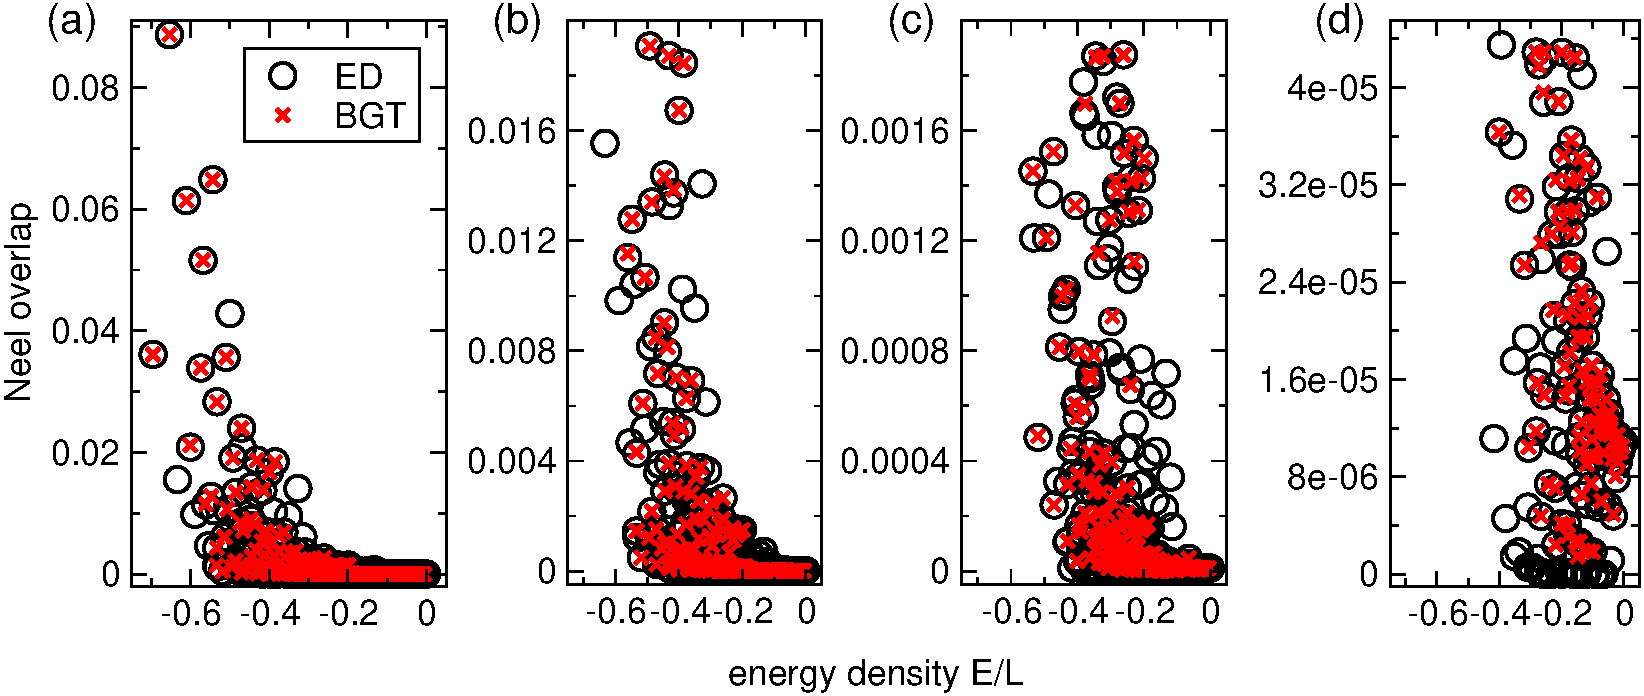
\includegraphics[width=.9\textwidth]{./draft_figs/L20_BT_check}
\end{center}
\caption{ The squared overlap $|\langle\Psi_0|\{\lambda\}\rangle|^2$ between the the 
 Neel state $|\Psi_0\rangle$ and the eigenstates $|\{\lambda\}\rangle$ of the $XXX$ 
 chain with $L=22$ sites. Only non-zero overlaps are shown. In all the panels the 
 $x$-axis shows the eigenstate energy density $E/L$. The circles are the exact 
 diagonalization results for all the non-zero overlaps. The crosses are the Bethe 
 ansatz results obtained using the Bethe-Gaudin-Takahashi equations. The missing 
 crosses correspond to eigenstates containing zero-momentum strings. (a) Overview 
 of all the non-zero overlaps. (b)(c)(d) The same overlaps as in (a) zooming in 
 the regions $[0,0.2]$, $[0,0.020]$, and $[0,4\cdot 10^{-5}]$. The discrepancies 
 between the ED and the Bethe ansatz results are attributed to the string deviations. 
}
\label{fig1-BGT-check}
\end{figure}
%##################################################################


%##################################################################
\begin{figure}[t]
\begin{center}
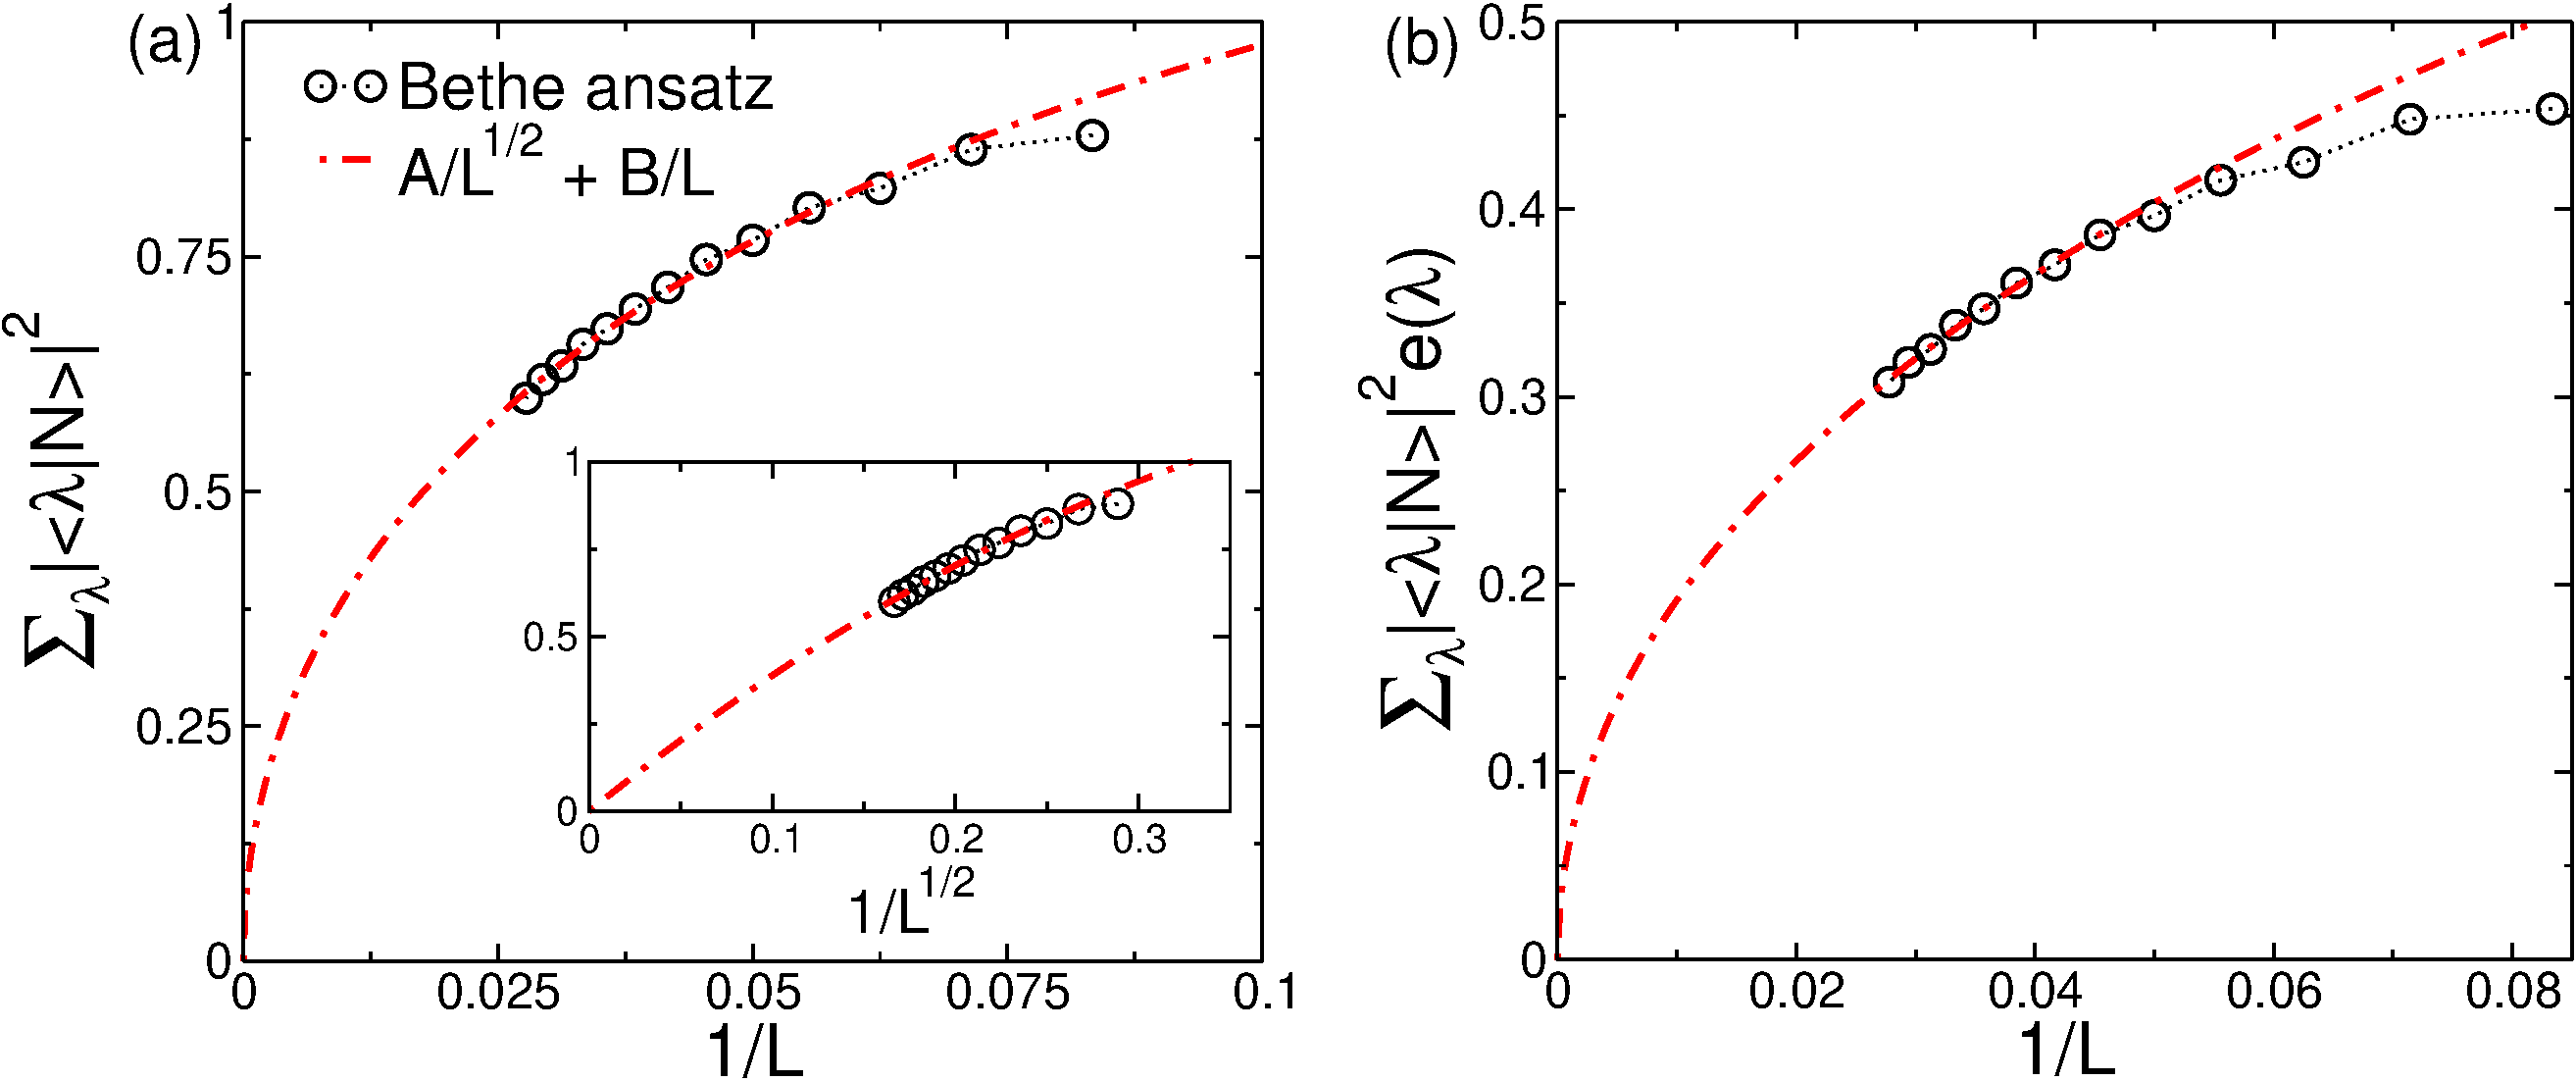
\includegraphics[width=.9\textwidth]{./draft_figs/Neel}
\end{center}
\caption{ Overlap sum rules for the Neel state. (a) The overlap sum rule 
 $\sum_{\{\lambda\}}|\langle\{\lambda\}|N\rangle|^2=1$, with $|N\rangle$ 
 the Neel state and $|\{\lambda\}\rangle$ the eigenstates  of the $XXX$ 
 spin chain. The $x$-axis shows $1/L$, with $L$ the chain length. The 
 circles are Bethe ansatz results for chains up to $L=36$. The results 
 are obtained via a full scanning of the chain Hilbert space. Only the 
 eigenstates with no zero-momentum strings are considered. The dash-dotted 
 line is a fit to $A/L^{1/2}+B/L$, with $A,B$ fitting parameters. Inset: 
 The same data as in the main Figure plotted versus $1/L^{1/2}$. (b) 
 The same as in (a) for the sum rule $\sum_{\{\lambda\}}|\langle\{
 \lambda\}|N\rangle|^2e(\{\lambda\})=1/2$, with $e(\{\lambda\})$  the 
 eigenstates energy density. 
}
\label{fig2-neel-sr}
\end{figure}
%##################################################################


%##################################################################
\begin{figure}[t]
\begin{center}
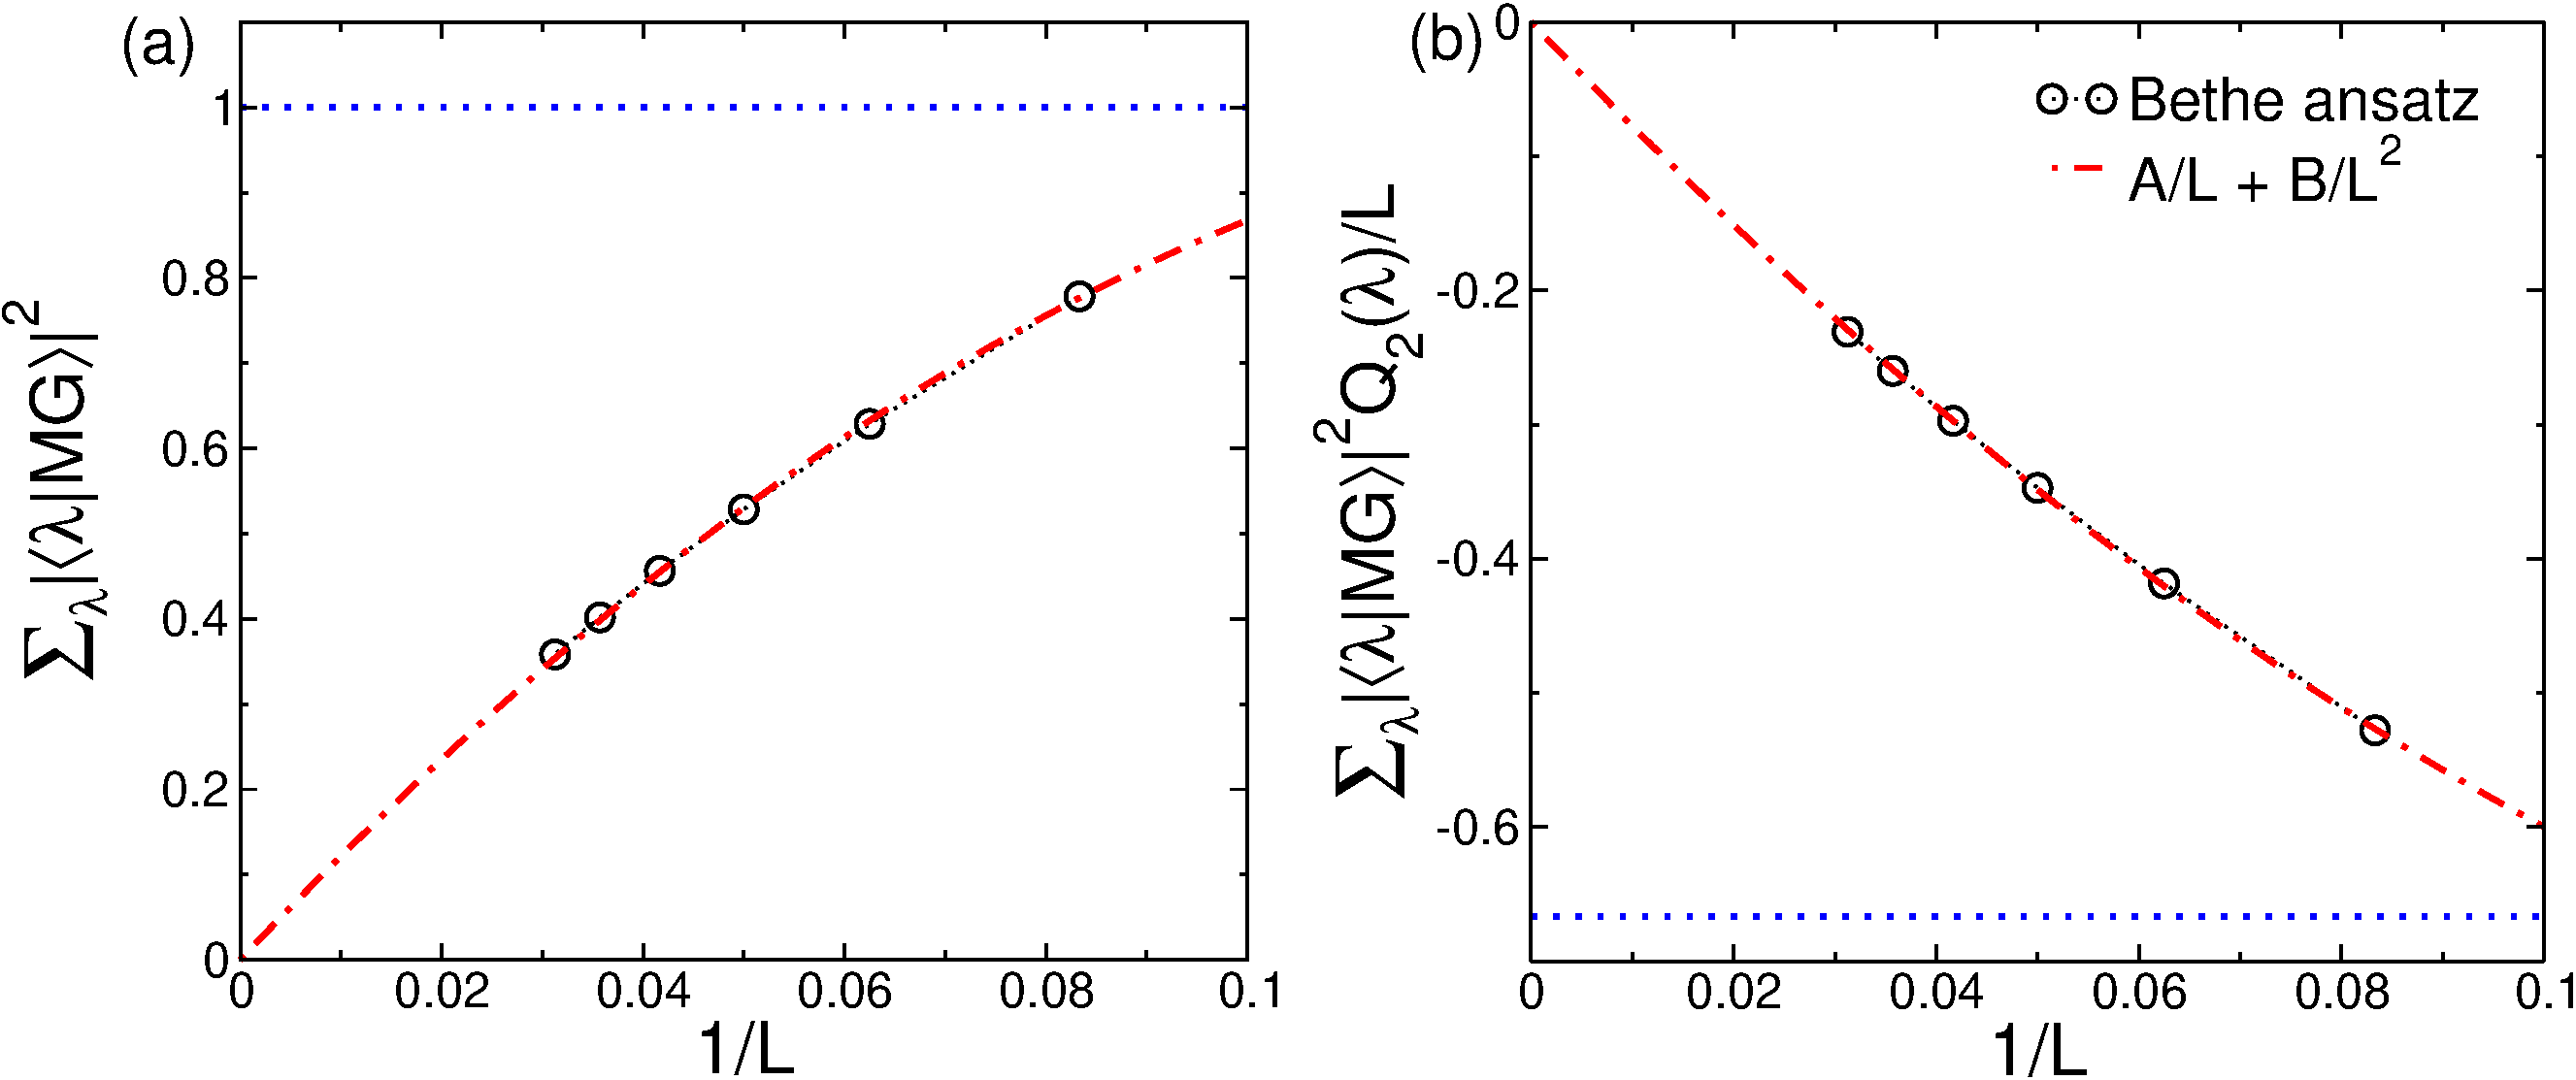
\includegraphics[width=.9\textwidth]{./draft_figs/Dimer}
\end{center}
\caption{ Overlap sum rules for the Majumdar-Ghosh (MG) state. (a) The 
 overlap sum rule $\sum_{\{\lambda\}}|\langle\{\lambda\}|MG\rangle|^2=1$, 
 with $|MG\rangle$ the Majumdar-Ghosh state and $|\{\lambda\}\rangle$ 
 the eigenstates  of the $XXX$ spin chain. The $x$-axis shows $1/L$, 
 with $L$ the chain length. The circles are Bethe ansatz results for 
 chains up to $L=36$. The results are obtained via a full scanning of 
 the chain Hilbert space. Only the eigenstates with no zero-momentum 
 strings are considered. The dash-dotted line is a fit to $A/L+B/L^2$, 
 with $A,B$ fitting parameters. (b) The same as in (a) for the sum 
 rule $\sum_{\{\lambda\}}|\langle\{\lambda\}|MG\rangle|^2e(\{\lambda\})=
 2/3$, with $e(\{\lambda\})$  the eigenstates energy density. 
}
\label{fig3-dimer-sr}
\end{figure}
%##################################################################


%##################################################################
\begin{figure}[t]
\begin{center}
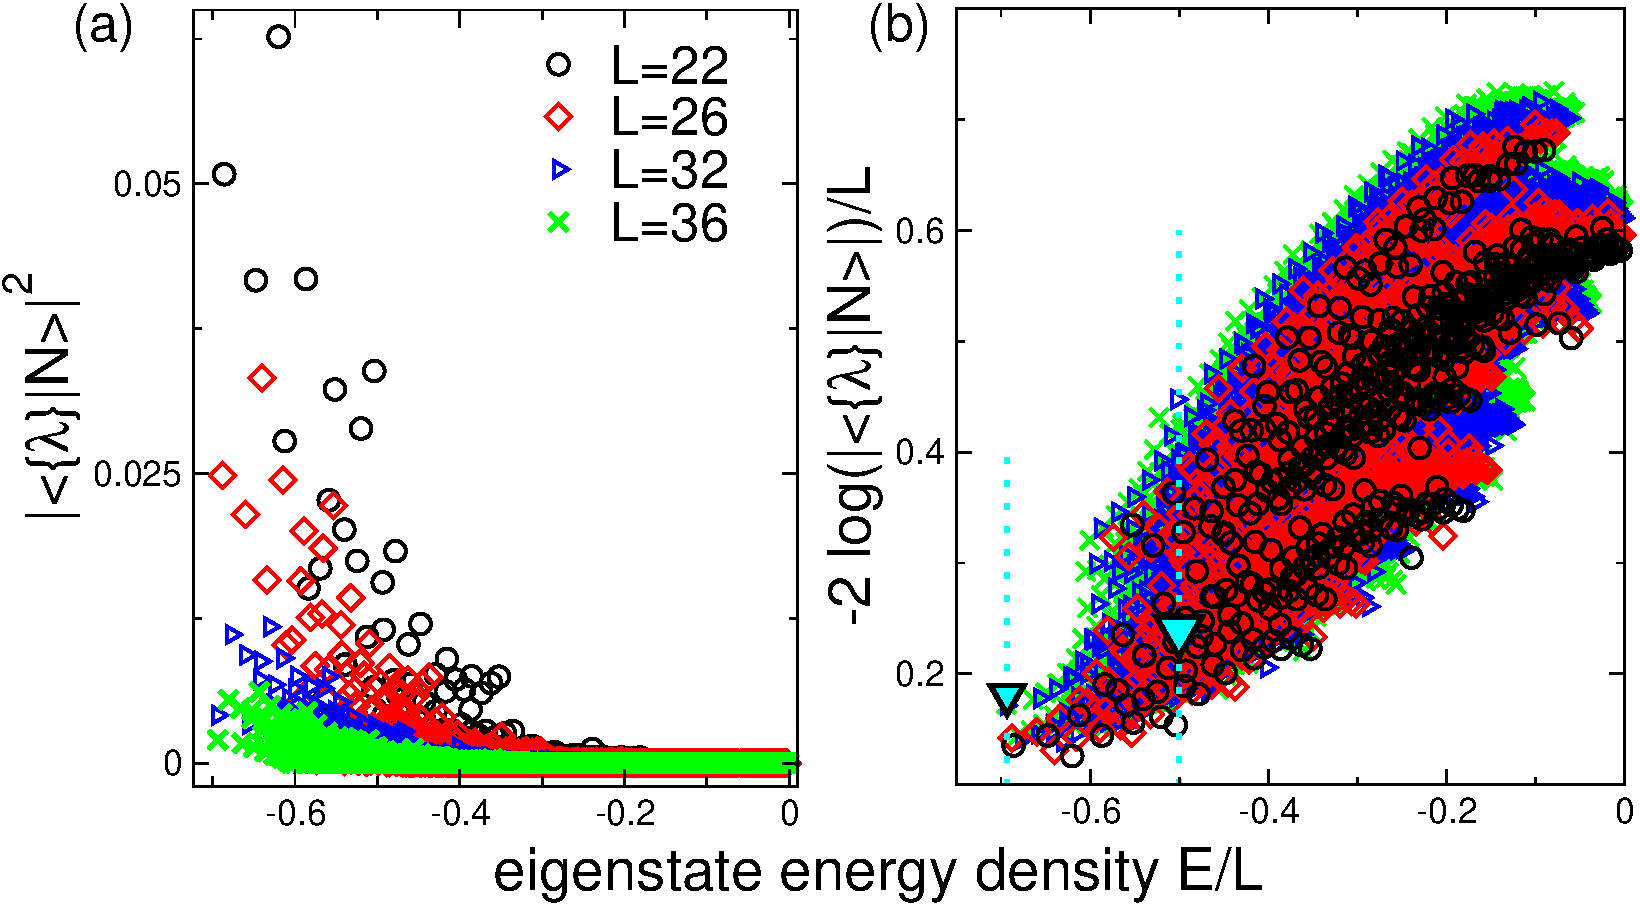
\includegraphics[width=.75\textwidth]{./draft_figs/Neel_over_ener}
\end{center}
\caption{ The overlap between the Neel state and the eigenstates of the 
 $XXX$ chain as a function of the eigenstate energy. (a) The squared 
 overlap $|\langle\{\lambda\}|Neel\rangle|^2$ plotted versus the 
 eigenstates energy density $E/L$. The data are Bethe ansatz results 
 for chains of length $L=22,26,32,36$ (different symbols). (b) Same as 
 in (a) plotting on the $y$-axis the combination $-2\log(|\langle\{
 \lambda\}|Neel\rangle|)/L$. 
}
\label{fig4-neel-ener}
\end{figure}
%##################################################################


%##################################################################
\begin{figure}[t]
\begin{center}
\includegraphics[width=.9\textwidth]{./draft_figs/QAMC_Obs_Neel}
\end{center}
\caption{ The overlap between the Neel state and the eigenstates of the 
 $XXX$ chain as a function of the eigenstate energy. (a) The squared 
 overlap $|\langle\{\lambda\}|Neel\rangle|^2$ plotted versus the 
 eigenstates energy density $E/L$. The data are Bethe ansatz results 
 for chains of length $L=22,26,32,36$ (different symbols). (b) Same as 
 in (a) plotting on the $y$-axis the combination $-2\log(|\langle\{
 \lambda\}|Neel\rangle|)/L$. 
}
\label{fig4-neel-ener}
\end{figure}
%##################################################################

%%%%%%
\subsection{Counting of eigenstates with non-zero Neel overlap}

We numerically checked that the number of states with non-zero overlap 
with the Neel state is given as 
%
\begin{equation}
\label{Neel-count}
Z_N=2^{\frac{L}{2}-1}+\frac{1}{2}B\left(\frac{L}{2},
\frac{L}{4}\right)+1,
\end{equation}
%
with $B(x,y)$ denoting the binomial coefficient. The contribution $1$ 
accounts for the ferromagnetic state. Here 
we assumed that $L$ is divisible by four. Here $Z_N$ is be obtained 
as the total number of parity-invariant Bethe-Gaudin-Takahashi quantum 
numbers. 

After excluding the zero-momentum strings the total number of states 
with non-zero overlap with the Neel state is 
%
\begin{equation}
\label{neel-ov-count}
Z'_{N}=B\left(\frac{L}{2},\frac{L}{4}\right)
\end{equation}
%
Importantly, the fraction of eigenstates corresponding to non-zero momentum 
strings is vanishing in the thermodynamic limit as 
%
\begin{equation}
\frac{Z_N'}{Z_N}\propto\frac{4}{\sqrt{\pi L}}.
\end{equation}
%
%%%%% PROOF
\subsection{Proof of~\eref{neel-ov-count}}

Here we prove~\eref{neel-ov-count}. The proof follows very closely the one of the 
completeness of the Bethe ansatz eigenstates {\bf cita qualcosa}. The proof is 
based on the counting of all the possible parity-invariant quantum number configurations. 

Given a generic $M$-particle eigenstate of the $XXX$ chain, due to parity invariance, 
if one excludes the zero-momentum strings only the $n$-strings with length $n\le M/2$ 
can contribute.

Thus, we denote the string content ${\mathcal S_{PI}}$ of a generic parity-invariant 
with no zero-momentum string eigenstate as ${\mathcal S}_{PI}\equiv\{s_1,\dots,s_{M/2}\}$.
Clearly one has the constraint $\sum_k ks_k=M/2$. We also restrict ourselves for simplicity 
to $L$ divisible by four. 

The number of available parity-invariant quantum numbers ${\mathcal N}_n$ in the $n$-string 
sector is given as  
%
\begin{equation}
{\mathcal N}_n(L,{\mathcal S}_{PI})=\frac{L}{2}-\sum_{m=1}^{M/2}t_{nm}s_m.
\end{equation}
%
Thus, the number of parity-invariant quantum number configurations ${\mathcal N}(L,{\mathcal 
S}_{PI})$ compatible with string content ${\mathcal S}_{PI}$ is obtained by choosing in 
all the possible ways the quantum numbers as  
%
\begin{equation}
{\mathcal N}(L,{\mathcal S}_{PI})=\prod_{k=1}^{M/2} B({\mathcal N}_k,s_k).
\end{equation}
%
It is useful to focus on the situation with fixed number of particles $0\le\ell\le M/2$ 
and number $1\le q\le M/2$ of independent strings. The total number of eigenstates 
${\mathcal N}''(L,\ell,q)$ is obtained as  
%
\begin{equation}
\label{eq}
{\mathcal N}''(L,\ell,q)=\sum\limits_{\{s_k\}\,s.t\, \sum k s_k=\ell, \sum s_k=q}{\mathcal N}(L,
{\mathcal S}_{PI}).
\end{equation}
%
where the sum is over all possible string contents $\{s_k\}$ compatible with the constraints 
$\sum_k s_k=q$ and $\sum_k k s_k=\ell$. 

The idea is now to derive a recursive relation for ${\mathcal N}''(L,\ell,q)$. 
It is useful to consider the shifted string content ${\mathcal S}'_{PI}$ as  
%
\begin{equation}
{\mathcal S}'_{PI}\equiv \{s_{m+1}\}\quad\textrm{with}\, s_m\in{\mathcal S}_{PI}.
\end{equation}
%
Observing that 
%
\begin{equation}
t_{ij}=t_{i-1,j-1}+2,
\end{equation}
%
one can write for $n>1$ that 
%
%\begin{eqnarray}
%{\mathcal N}_n(L,{\mathcal S}_{PI})=\Big\lceil\frac{L}{2}-\frac{1}{2}\Big\rceil-t_{n,1}s_1-
%\sum\limits_{m>1}t_{nm}s_m=\\
%\Big\lceil\frac{L}{2}-\frac{1}{2}\Big\rceil-2s_1-
%\sum\limits_{m>1}(t_{n-1,m-1}+2)s_m=\\
%\Big\lceil\frac{L}{2}-\frac{1}{2}\Big\rceil-2q-
%\sum\limits_{m}t_{n-1,m}s'_m.
%\end{eqnarray}
%
%This means
%
\begin{equation}
{\mathcal N}_n(L,{\mathcal S}_{PI})={\mathcal N}_{n-1}(L-4q,{\mathcal S}'_{PI}),
\end{equation}
%
which implies
%
\begin{equation}
Z(L,{\mathcal S})=B(Z_1(L,{\mathcal S}),s_1)Z(L-4q,{\mathcal S}').
\end{equation}
%
Substituting in~\eref{eq} one obtains
%
\begin{equation}
Z(L,\ell,q)=\sum_{s=0}^{q-1}B\Big(\Big\lceil\frac{L}{2}-\frac{1}{2}\Big
\rceil-2q+s,s\Big)Z(L-4q,\ell-q,q-s),
\end{equation}
%
i.e.,
%
\begin{equation}
Z(L,\ell,q)=\sum_{s=0}^{q-1}B\Big(\frac{L}{2}-2q+s,s\Big)Z(L-4q,\ell-q,q-s).
\end{equation}
%
The initial condition $Z(L,1,1)$ reads 
%
\begin{equation}
Z(L,1,1)=\frac{L}{2}-1
\end{equation}
%
One can show that this leads to 
%
\begin{equation}
Z(L,\ell,q)=\frac{L/2-2\ell+1}{L/2-\ell+1}B(L/2-\ell+1,q)B(\ell-1,q-1).
\end{equation}
%
By summing over $q=1,\dots,\ell$ one obtains 
%
\begin{equation}
\sum\limits_{q=1}^\ell Z(L,\ell,q)=B(L/2,\ell)-B(L/2,\ell-1).
\end{equation}
%
Summing over $\ell$ one obtains~\eref{neel-ov-count}.


%%%%%%%%%%%%%
\subsection{Proof of non-zero Neel overlap counting}

Here we prove~\eref{Neel-count}. 

Let us consider the string configurations as before in which all the particle are 
distributed in at most $M/2$-strings, as ${\mathcal S}_{PI}=\{s_1,s_2,\dots,s_{M/2}\}$. 
Now we have $\sum_k ks_k=M$. 

The number of available parity-invariant quantum numbers ${\mathcal N}_n$ in the 
$n$-string sector is now given as 
%
\begin{equation}
{\mathcal N}_n(L,{\mathcal S}_{PI})=\left\lfloor\frac{L}{2}-\frac{1}{2}
\sum_{m=1}^{M/2}t_{nm}s_m\right\rfloor.
\end{equation}
%
Thus, the number of parity-invariant quantum number configurations ${\mathcal N}(L,{\mathcal 
S}_{PI})$ compatible with string content ${\mathcal S}_{PI}$ is obtained by choosing in 
all the possible ways the quantum numbers as  
%
\begin{equation}
{\mathcal N}(L,{\mathcal S}_{PI})=\prod_{k=1}^{M/2} B\left({\mathcal N}_k,\left\lfloor\frac{s_k}{2}
\right\rfloor\right).
\end{equation}
%
We focus now to the situation with fixed number of particles $0\le\ell\le M/2$ and number 
$1\le q\le M/2$ of independent strings. 

The total number of eigenstates is given as 
%
\begin{equation}
\label{eqq}
{\mathcal N}''(L,\ell,q)=\sum\limits_{\{s_k\}\,s.t\, \sum k s_k=\ell, \sum s_k=q}{\mathcal N}(L,
{\mathcal S}_{PI}).
\end{equation}
%
where the sum is over all possible string contents $\{s_k\}$ compatible with the constraints 
$\sum_k s_k=q$ and $\sum_k k s_k=\ell$. 

The idea is now to derive a recursive relation for ${\mathcal N}''(L,\ell,q)$. 
It is useful to consider the shifted string content ${\mathcal S}'_{PI}$ as  
%
\begin{equation}
{\mathcal S}'_{PI}\equiv \{s_{m+1}\}\quad\textrm{with}\, s_m\in{\mathcal S}_{PI}.
\end{equation}
%
Observing that 
%
\begin{equation}
t_{ij}=t_{i-1,j-1}+2,
\end{equation}
%
one can write for $n>1$ that 
%
\begin{equation}
{\mathcal N}_n(L,{\mathcal S}_{PI})={\mathcal N}_{n-1}(L-2q,{\mathcal S}'_{PI}),
\end{equation}
%
which implies that 
%
\begin{equation}
Z(L,{\mathcal S})=B(Z_1(L,{\mathcal S}),\lfloor s_1/2\rfloor)Z(L-2q,{\mathcal S}')
\end{equation}
%
One then has 
%
\begin{equation}
Z(L,\ell,q)=\sum_{s=0}^{q-1}B\Big(\frac{L}{2}-q+\left\lfloor\frac{s}{2}\right\rfloor,
\left\lfloor\frac{s}{2}\right\rfloor\Big)Z\left(L-2q,\ell-q,
q-s\right).
\end{equation}
%
The initial condition $Z(L,1,1)$ reads 
%
\begin{equation}
Z(L,1,1)=\frac{L}{2}-1
\end{equation}
%












\begin{table}[h]
\scriptsize
\centering
Bethe states with nonzero N\'eel overlap ($N=12$)\\[1ex]
\begin{tabular}{rrrrr}
String content & $2I^+_n$ & E & $|\langle \{\lambda\}| \Psi_0 \rangle|^2$ & here \\[0.3em]
\toprule
6 inf & - & $0$ & $0.002164502165$ & $0.002164502165$ \\
\midrule
2 one, 4 inf &$1_1 $ & $-3.918985947229$ & $0.096183409244$ & $0.096183409244237$ \\
 &$3_1 $ & $-3.309721467891$ & $0.011288497947$ &  $0.0112884979464673$\\
 &$5_1 $ & $-2.284629676547$ & $0.004542580506$ &  $0.0045425805061850$\\
 &$7_1 $ & $-1.169169973996$ & $0.002752622983$ &  $0.0027526229835876$\\
 &$9_1 $ & $-0.317492934338$ & $0.002116006203$ &  $0.0021160062026402$\\
\midrule
4 one, 2 inf &$1_1 3_1 $ & $-7.070529325964$ & $0.310133033838$ &$ 0.554809782804$ \\
  &$1_1 5_1 $ & $-5.847128730477$ & $0.129277023687$ \\
  &$ 1_1 7_1$ & $-4.570746557876$ & $0.085992436024$ \\
  &$ 3_1 5_1$ & $-5.153853093221$ & $0.015256395523$ \\
  &$3_1 7_1 $ & $-3.916336243695$ & $0.010091113504$ \\
  &$5_1 7_1 $ & $-2.817696043731$ & $0.004059780228$ \\
  \midrule
2 two, 2 inf &$1_2 $ & $-1.905667167442$ & $0.001207238321$ & $0.005468702625$\\
  &$3_2 $ & $-1.368837200825$ & $0.002340453815$ \\
  &$5_2 $ & $-0.681173793635$ & $0.001921010489$ \\
    \midrule
1 one, 1 three, 2 inf &$0_1 0_3 $ & $-2.668031843135$ & $0.034959609810$ & $0.034959609810$ \\
    \midrule
6 one &$1_1 3_1 5_1 $ & $-8.387390917445$ & $0.153412152966$ & $0.153412152966$ \\
  \midrule
2 two, 2 one &$1_1 1_2 $ & $-5.401838225870$ & $0.040162686361$ & $0.046134750850$ \\
  &$3_1 1_2 $ & $-4.613929948329$ & $0.004636541934$ \\
  &$5_1 1_2 $ & $-3.147465758841$ & $0.001335522556$ \\
    \midrule
1 three, 3 one &$0_1 2_1 0_3$ & $-6.340207488736$ & $0.052743525774$ & $0.078910020729$ \\
  &$0_1 4_1 0_3$ & $-5.203653009936$ & $0.015022005621$ \\
  &$0_1 6_1 0_3$ & $-3.788693957250$ & $0.011144489334$ \\
      \midrule
1 five, 1 one &$0_1 0_5$ & $-2.444293750583$ & $0.005887902992$ & $0.005887902992$ \\
      \midrule
2 three &$1_3$ & $-1.111855930538$ & $0.001342476001$ & $0.001342476001$ \\
      \midrule
1 two, 1 four &$0_2 0_4$ & $-1.560671012472$ & $0.000026982174$ & $0.000026982174$ \\
  \bottomrule
 \end{tabular}
\caption{All Bethe states for $N=12$ with nonzero overlap with the zero-momentum N\'eel state. The 
overlap squares add up to $1$ up to the precision in which the Bethe equations were solved. The 
$2I^+_n$ in the second column give the positive $n$-string quantum numbers of the parity-invariant 
Bethe states.}
\label{table:RV:sumruleN12}
\end{table}

\begin{table}[h]
\scriptsize
\centering
Bethe states with nonzero M-G overlap ($L=12$)\\[1ex]
\begin{tabular}{rrrr}
String content & Energy (ED) & $|\langle \{\lambda\}| \Psi_0 \rangle|^2$ (ED) & $|\langle \{\lambda\}| \Psi_0 \rangle|^2$ (B-T) \\[0.3em]
\toprule
$1_1 3_1 5_1$ & $-8.38739$  & $0.716616$     &  $0.7166157692239$\\
              & $-6.34021$  & $0.205891$     &  \\
$5_1 1_2$     & $-5.40184$  & $0.0556247$    & $0.05403336654338$\\
              & $-5.20365$  & $0.0388322$    & \\
$3_1 1_2$     & $-4.61393$  & $0.00568743$   & $0.005582983043235$\\
              & $-3.78869$  & $0.00601941$   & \\
$1_1 1_2$     & $-3.14747$  & $0.00210748$   & $0.0021070869333835$\\
              & $-2.44429$  & $0.000129601$  & \\
              & $-1.56067$  & $0.000330573$  & \\
$1_3$         & $-1.11186$  & $0.0000117278$ & $0.000012785579923275$\\
\bottomrule
\end{tabular}
\caption{All Bethe states for $L=12$ with nonzero overlap with the zero-momentum 
 M-G state. The first column show the string content of the eigenstate. The second 
 and third columns show the exact diagonalization resutls for the energy and the 
 overlap, respectively. The last colum is the overlap obtained in the Bethe ansatz 
 approach using the Bethe-Takahashi equations.
}
\label{table:RV:sumruleN12}
\end{table}


\begin{table}[h]
\scriptsize
\centering
Bethe states with nonzero M-G overlap ($L=16$)\\[1ex]
\begin{tabular}{rrrr}
String content & Energy (ED) & $|\langle \{\lambda\}| \Psi_0 \rangle|^2$ (ED) & $|\langle \{\lambda\}| \Psi_0 \rangle|^2$ (B-T) \\[0.3em]
\toprule
$7_1 5_1 3_1 1_1$ & $-11.1423$ & $0.517742$         & $0.5177418283152$\\
& $-9.59129$ & $0.244845$         &\\
$7_1 5_1 1_2$ & $-8.81424$ & $0.0727096$        & $0.07100180464371$\\
& $-8.56579$ & $0.082852$         &\\
$7_1 3_1 1_2$ & $-7.96995$ & $0.0232953$        & $0.02300602650371$\\
& $-7.89112$  & $0.0181713$        &\\
$7_1 1_1 1_2$ & $-7.51522$ & $0.00245007$       & $0.002427999643379$\\
& $-7.41983$ & $0.0192443$        &\\
$5_1 3_1 1_2$ & $-6.80829$ & $0.012519$         & $0.012518660407092$\\
& $-6.78357$ & $0.00398018$       &\\
$5_1 1_1 1_2$ & $-6.3398$  &  $0.00135119$      & $0.0013511980854654$\\
& $-6.25276$ & $0.000721952$      &\\
& $-5.86683$ & $0.00112415$       &\\
& $-5.69103$ & $0.000141052$      &\\
& $-5.50802$ & $0.00373666$       &\\
$3_1 1_2$ & $-5.45276$ & $0.000466819$      & $0.0004668223478716$\\
& $-5.06385$ & $0.000380056$      & $0.000166548883431$\\
& $-4.86668$ & $0.0000395855$     &\\
& $-4.64743$ & $0.000014786$      & $0.000016403668846624$\\
& $-4.49059$ & $0.00155894$       &\\
& $-4.25924$ & $0.000109932$      &\\
& $-3.93068$ & $4.12108e-6$       & $4.6283550855711e-6$\\
& $-3.92645$ & $0.0000102752$     &\\
& $-3.77995$ & $0.0000732808$     &\\
& $-3.259$   & $0.0000348879$     &\\
& $-3.12751$ & $0.0000739906$     & $0.00007017294942524$\\
& $-3.04176$ & $1.62543e-6$       &\\
& $-3.00072$ & $1.4684e-6$        & $1.6374806913113e-6$\\
& $-2.32465$ & $2.01172e-8$       &\\
& $-2.26529$ & $7.53377e-6$       &\\
& $-2.02465$ & $5.8028e-7$        & $5.722094498217e-7$\\
& $-1.38078$ & $2.17607e-7$       &\\
& $-1.11438$ & $1.825e-7$         &\\
& $-0.844856$& $1.84715e-9$       & $2.4957509639475e-9$\\
\bottomrule
\end{tabular}
\caption{All Bethe states for $L=12$ with nonzero overlap with the zero-momentum 
 M-G state. The first column show the string content of the eigenstate. The second 
 and third columns show the exact diagonalization resutls for the energy and the 
 overlap, respectively. The last colum is the overlap obtained in the Bethe ansatz 
 approach using the Bethe-Takahashi equations.
}
\label{table:RV:sumruleN12}
\end{table}



%%%%%%%%%%%%%%%%%%%%%% REFERENCES %%%%%%%%%%%%%%%%%%%%%%%%%%%%%%%%%%%%%%%%%%%%%%%%

\begin{thebibliography}{99}

\bibitem{calabrese-2014}
P.~Calabrese and P.~Le Doussal, J.\ Stat.\ Mech.\ (2014) P05004. 

\end{thebibliography}


\end{document}


